\documentclass[12pt,fleqn]{article}
\usepackage{xiiiemc}
\usepackage{natbib}
\usepackage{fancyhdr}
\usepackage{fancyvrb}
\usepackage{color}
\usepackage{wallpaper} 
\usepackage{titlesec}   %% Define space between paragraph e section
\usepackage{float} 	%% Use to fix Figure or Table: ex: \begin{table}[H]
\usepackage[usenames,dvipsnames]{xcolor}
\usepackage{hyperref} 	%% Use to fix Figure or Table: ex: \begin{table}[H]
\hypersetup{
	%pagebackref=true,
	pdfcreator={LaTeX with abnTeX2},
	pdfkeywords={abnt}{latex}{abntex}{USPSC}{trabalho acadêmico}, 
	colorlinks=true,       		% false: boxed links; true: colored links
	linkcolor=blue,          	% color of internal links
	citecolor=blue,        		% color of links to bibliography
	filecolor=magenta,      		% color of file links
	urlcolor=blue,
	allbordercolors=black,
	bookmarksdepth=4
}
\usepackage{tocloft}
\titleformat{\section}
  {\normalfont\bfseries}{\thesection.}{0.5em}{}
\renewcommand\cftsecaftersnum{.} 
\renewcommand\thesection{\arabic{section}}
\renewcommand\thesubsection{\thesection.\arabic{subsection}}
%%%%Don't edit this block. It reduces the spacing between the lines of the references
\let\OLDthebibliography\thebibliography
\renewcommand\thebibliography[1]{\OLDthebibliography{#1} \setlength{\parskip}{0pt}\setlength{\itemsep}{0pt plus 0.3ex}}

\usepackage{grffile}
\usepackage{afterpage}

%%-----------------------------------------------EDIT-----------------------------------------------
\title{A distance derived from the Kolmogorov-Smirnov statistic:
	specification, reference measures and example uses}

%%-----------------------------------------------EDIT----------------------------------------------
\author
    {\rm \begin{tabular}{l} 
    \textbf{Renato Fabbri}$$ - {\textnormal renato.fabbri@gmail.com}\\%
    {\fontsize{11}{0}\selectfont University of São Paulo, Institute of Mathematical and Computer Sciences - São Carlos, SP, Brazil}\vspace*{-0.05cm} \\
%    {\fontsize{11}{0}\selectfont $^{2}$Federal University of ABC, Centre for Natural Sciences and Humanities - São Paulo, SP, Brazil}\vspace*{-0.05cm}\\
  \end{tabular}}
%%----------------------------------------------------------------------------------------------

\fancypagestyle{firspagetstyle}
{
	\lhead{}
	\fancyhead[C]{%
		
\includegraphics[width=0.9\linewidth]{logo}\\%
		{\scriptsize \fontfamily{phv}\fontseries{b}\selectfont \color[rgb]{0.45,0.45,0.45}
		16 a 19 de Outubro de 2017\\
		Instituto Politécnico - Universidade do Estado de Rio de Janeiro\\
		Nova Friburgo - RJ\\
	    }
	}
	\renewcommand{\headrulewidth}{0.0pt}
	\fancyfoot[C]{\footnotesize \parbox{15cm} {\centering  \fontsize{7.5}{0}\selectfont \it Anais do XX ENMC – Encontro Nacional de Modelagem Computacional e VIII ECTM – Encontro de Ciências e Tecnologia de Materiais,  Nova Friburgo, RJ – 16 a 19 Outubro 2017}} % \ttfamil
	\rhead{}
}


\begin{document}
\maketitle

\thispagestyle{firspagetstyle}

\fancyhead[L]{\footnotesize{\fontsize{7.5}{0}\selectfont \it XX ENMC e VIII ECTM\\
	16 a 19 de Outubro de 2017\\
	Instituto Politécnico Universidade do Estado do Rio de Janeiro – Nova Friburgo - RJ\\}}
\renewcommand{\headrulewidth}{0.0pt}
\fancyfoot[C]{\footnotesize \parbox{15cm} {\centering  \fontsize{7.5}{0}\selectfont \it Anais do XX ENMC – Encontro Nacional de Modelagem Computacional e VIII ECTM – Encontro de Ciências e Tecnologia de Materiais,  Nova Friburgo, RJ – 16 a 19 Outubro 2017}} % \ttfamil
\rhead{}

\begin{abstract}
Statistical distances quantifies the difference between two statistical constructs.
In this article, we describe reference values for a semimetric
derived from the Kolmogorov-Smirnov statistic $D_{F,F'}$.
Each measure of the $D_{F,F'}$ is a distance between two histograms.
This distance is normalized by the number of observations in each sample
to yield the $c'=D_{F,F'}\sqrt{\frac{n n'}{n+n'}}$ statistic,
which can be mapped to p-values, i.e. values for which 
high enough levels of significance $\alpha$ implies the rejection of the
	null hypothesis (that the samples are drawn from the same distribution).
One great feature of $c'$ is that it inherits the robustness of
	$D_{F,F'}$ and is thus suitable for use in settings where
	the underlying distributions are not known.
Benchmarks are derived by comparing samples from standard distributions.
The supplied example applications of the $c'$ statistic for the distinction
	of samples in real data enables further
insights about the robustness and power of $c$.
\end{abstract}

\keywords{\em{Statistical distance, Statistics, Kolmogorov-Smirnov test, Statistical test, Benchmark}}

\pagestyle{fancy}

\section{INTRODUCTION}\label{sec:intro}
To quantify the difference between samples that are regarded as statistical events,
one can rely in statistical distances.
Such distances are often not metrics, cases in which they fail in one of
the properties of a metric $m$ on sets $x_i \in X$:
\begin{align}
	m(x_i,x_j) &  \geq 0 \\
	m(x_i,x_j) &  = 0 \Leftrightarrow x_i = x_j \\
	m(x_i,x_j) &  = m(x_j,x_i)\\
	m(x_i,x_j) &  \leq m(x_i,x_z) + m(x_z,x_j)
\end{align}

Pseudometrics violate property (1) and/or (2),
quasimetrics violate property (3),
semimetrics violate property (4).
A divergence only satisfies properties (1) and (2).
These are ``generalized metrics''.

In this article, a statistical distance derived from the
Kolmogorov-Smirnov statistic is described.
To enable the use of the (generalized) metric,
benchmarks are provided
by using standard distributions in various settings and sample sizes.
Example applications of the metric to quantify the difference among
real signals further validate the approach.

Section~\ref{sec:met} describe the metric
and the methods used to characterize it.
Section~\ref{sec:res} is dedicated to
summarizing the results and essential discussions.
Final remarks, including potential future works,
are stated in Section~\ref{sec:res}.


\section{METHODS}\label{sec:met}
This section describes the $c'$ statistical distance,
the strategy of benchmarking and to validate $c'$ by means
of application to real samples.


\subsection{Description of the $c'$ statistic}
Be $F$ and $F'$ two empirical cumulative distributions,
where $n$ and $n'$ are the number of observations in each sample.
The two-sample Kolmogorov-Smirnov test rejects the null hypothesis,
that the histograms are the outcome of the same underlying distribution,
if:
\begin{equation}\label{eq:ks}
D_{F,F'} > c(\alpha)\sqrt{\frac{n+n'}{nn'}}
\end{equation}

\noindent where $D_{F,F'}=sup_x[F-F']$ as in Figure~\ref{fig:dnn}
and $c(\alpha)$ is related to the level of significance $\alpha$ by:

\begin{table}[h!]
\centering
\begin{tabular}{|l||c|c|c|c|c|c|}\hline
$\alpha$    & 0.1  & 0.05 & 0.025 & 0.01 & 0.005 & 0.001 \\\hline
$c(\alpha)$ & 1.22 & 1.36 & 1.48  & 1.63 & 1.73  & 1.95  \\\hline
\end{tabular}
\end{table}

If distributions are drawn from empirical data, $D_{F,F'}$ is given as are $n$ and $n'$.
All terms in equation~\ref{eq:ks} are positive and $c(\alpha)$ can be isolated:

\begin{equation}\label{eq:ks2}
%	c(\alpha) < \frac{D_{F,F'}}{\sqrt{\frac{n+n'}{nn'}}} = c
	c(\alpha) < D_{F,F'}\sqrt{\frac{nn'}{n+n'}} = c'
\end{equation}

%Tables~\ref{tab:kolSub}-\ref{tab:kolPctInter} are populated with values for $c'(\alpha)$
The higher $c'$ is, the lower $\alpha$ can be and still entail the rejection of the null hypothesis.

\begin{figure}[!h]
	\centering
	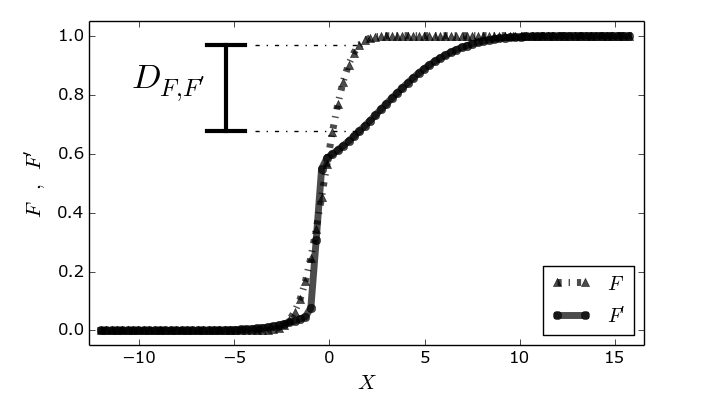
\includegraphics[width=0.44\textwidth]{../figs/Dnn}
	\caption{The Kolmogorov-Smirnov statistic $D_{F,F'}$: the maximum difference between
		two cumulative distribution functions.}
	\label{fig:dnn}
\end{figure}

In summary,
high values of $c$ favor rejecting the null hypothesis.
For example, if the significance level is $\alpha=0.01$,
then $c'$ greater than $1.7$
implies the rejection of the null hypothesis,
i.e. assuming that $F$ and $F'$
are outcomes of different distributions.

Of core importance in this study is to regard $c'$
as a measure of distance between both distributions~\cite{kolm}.
If fact, it is a statistical distance.
Following the concepts defined in Section~\ref{sec:intro},
it is a generalized metric.
It obviously satifies the Equations (1) and (3).
But it violates Equation (2) and satisfies Equation (4) for less obvious reasons.
The obtainance of $c'$ depends on making histograms,
thus if a slightly different observation of a sample lies on the same bin,
$c'=m(x_i,m_j) = 0$  and $x_i \neq x_j$, which violates (2).
If we instead regard $x_i$ as a histogram, not a sample,
that it satifies (2), but we here assume that we want 
To grasp how $c'$ satisfies Equation (4),
let $x_i$, $x_j$ and $x_z$ be samples of the same size,
so we only need to compare the $D_{F,F'}$.
Let $F_i$ be the cumulative distribution of the sample $x_i$.
Supose that in the value $\xi$ of X where $F_i$ and $F_j$ are maximally different (i.e. where they yield $D_{F_i,F_j}$),
they are also maximaly different against $F_z$.
If the value of $F_z(\xi)$ is between $F_x(\xi)$ and $F_j(\xi)$:
$D_{F_i,F_z}+D_{F_j,F_z} = D_{F_i,F_j}$,
otherwise:
$D_{F_i,F_z}+D_{F_j,F_z} > D_{F_i,F_j}$.
If the KS statistic $D_{F,F'}$ are not yield at the same sample value,
it is because they are larger than in the previous cases, thus:
$D_{F_i,F_z}+D_{F_j,F_z} > D_{F_i,F_j}$.
And this completes the argument for:
$D_{F_i,F_z}+D_{F_j,F_z} \geq D_{F_i,F_j}$.


% discrete vs continous

% are histograms really needed?



\subsection{Philosophical and technological note}
Difference and equivalence is of central role in human cognition,
philosophy and science.
This fact is so deeply recognized that thinkers often reduce
thought to classifications, e.g. through the
mathematical concept of equivalence classes~\cite{deleuze}.
Histograms are very immediate and informative
roughly wherever there is a phenomenon of interest which can yield measurements.
This present document should enable conclusions to be drawn about 
the equivalence (and difference)
of the processes underlying sets of measurements for a very
broad range of phenomena.
The following tables 
also validate the mathematical framework
and the software implementation.

\subsection{Document outline}
Section~\ref{sec:simulations} exposes reference values drawn from simulations.
Section~\ref{sec:empirical} exemplifies the use of the $c$ statistic
to make sense of phenomena.
Section~\ref{sec:conc} holds final remarks with directions to
software and data.



\subsection*{\textit{Acknowledgements}}
The authors thank CNPq and FAPESP for the funding received while researching the topic of this article,
the researchers of IFSC/USP and ICMC/USP for the recurrent collaboration in every situation
where we needed directions for investigation.

% ------------------------------------------------------------------------
\begin{thebibliography}{99}
\fontsize{11}{0}\selectfont
\bibitem[Fabbri, 2017]{enhance}
	Fabbri, R. (2017). Enhancements of linked data expressiveness for ontologies.
		Encontro Nacional de Modelagem Computacional 2017 (XX ENMC).
		From \url{https://github.com/ttm/ontologyEnhancements/raw/master/article.pdf}

\bibitem[Heath \& Bizer, 2011]{ldb}
	Heath, T. \& Bizer, C. (2011). Linked Data: Evolving the Web into a Global Data Space (1st edition). Synthesis Lectures on the Semantic Web: Theory and Technology, 1:1, 1-136. Morgan \& Claypool.

\bibitem[Lehmann et al., 2015]{dbpedia}
	Lehmann, J., Isele, R., Jakob, M., Jentzsch, A., Kontokostas, D., Mendes, P. N., ... \& Bizer, C. (2015). DBpedia–a large-scale, multilingual knowledge base extracted from Wikipedia. Semantic Web, 6(2), 167-195.

\bibitem[Munzner, 2014]{munzner}
	Munzner, T. (2014). Visualization analysis and design. CRC press.

\bibitem[W3C, 2010]{w3cld}
	W3C (2017). LINKED DATA CURRENT STATUS, from \url{https://www.w3.org/standards/techs/linkeddata}

\bibitem[Ward et al., 2010]{ward}
	Ward, M. O., Grinstein, G., \& Keim, D. (2010). Interactive data visualization: foundations, techniques, and applications. CRC Press.

\bibitem[Wikipedia, 2017]{wikipData}
	Data. (2017, August 21). In Wikipedia, The Free Encyclopedia. Retrieved
		22:31, August 21, 2017
		, from \url{https://en.wikipedia.org/w/index.php?title=Data&oldid=796493851}

\end{thebibliography}
% ------------------------------------------------------------------------

%For papers written in Portuguese or Spanish.

%\begin{center}
%  TITLE IN ENGLISH
%\end{center}

%\def\abstractname{Abstract}%

%\begin{abstract}
%   Abstract in english
%\end{abstract}

%\keywords{\em{Keywords in english}}

\end{document}
